\documentclass[runningheads]{llncs}
%
\usepackage[T1]{fontenc}
\usepackage{graphicx}
\usepackage{amsmath}
\usepackage{amssymb}
\usepackage{hyperref}
\usepackage{booktabs}
\usepackage{listings}
\usepackage{xcolor}
\usepackage[section]{placeins}

% Tighter float spacing
\setlength{\textfloatsep}{8pt plus 2pt minus 4pt}
\setlength{\floatsep}{6pt plus 2pt minus 2pt}
\setlength{\intextsep}{8pt plus 2pt minus 4pt}
\renewcommand{\topfraction}{0.85}
\renewcommand{\bottomfraction}{0.70}
\renewcommand{\textfraction}{0.10}
\renewcommand{\floatpagefraction}{0.65}

% Listings style for NormCode snippets
\lstset{
  basicstyle=\ttfamily\small,
  breaklines=true,
  frame=single,
  backgroundcolor=\color{gray!8},
  rulecolor=\color{gray!40},
  xleftmargin=6pt,
  xrightmargin=6pt,
}

\begin{document}

\title{NormCode Canvas as a Case-Based Reasoning Development Platform\\for Large Language Model Agentic Workflows}

\titlerunning{NormCode Canvas: CBR Development Platform for LLM Agentic Workflows}

\author{Anonymous Author(s)}
\authorrunning{Anonymous}

\institute{Anonymous Institution\\
\email{anonymous@anonymous.org}}

\maketitle

%----------------------------------------------------------------
\begin{abstract}
We present \textbf{NormCode Canvas} (v1.1.3), a deployed system realizing
Case-Based Reasoning at two levels for multi-step LLM workflows. The foundation
is NormCode \cite{anon2025}, a semi-formal planning language whose compiler-verified
scope rule ensures every execution checkpoint is a genuinely self-contained case ---
eliminating the implicit shared state that makes retrieval unreliable and failure
non-localizable in standard orchestration frameworks.
\textbf{Level~1} treats each checkpoint as a concrete case (suspended runtime:
Blackboard + Concept Repository snapshot); Fork implements retrieve-and-reuse, Value
Override implements revision with automatic stale-boundary propagation.
\textbf{Level~2} treats each compiled plan as an abstract case; four production-ready
plans demonstrate domain generality, and the compiler is itself a NormCode plan
enabling recursive case learning.
Three structural properties follow: \textbf{(C1)} failure localization in O(1)
operations; \textbf{(C2)} pre-execution review via compiler-generated narrative;
\textbf{(C3)} scope-bounded selective re-execution.
Two case studies illustrate both levels in practice.

\keywords{case-based reasoning \and LLM workflows \and AI workflow development
\and workflow management \and agents \and LLM reasoning \and agent DSL}
\end{abstract}

%================================================================
\section{Introduction}
\label{sec:intro}

Multi-step LLM workflows---where each inference step feeds the next---have emerged as a
standard architecture for deploying language models in real applications. Frameworks such
as LangChain \cite{chase2022}, LangGraph \cite{langgraph2024}, AutoGen \cite{wu2023},
and PromptFlow \cite{microsoft2023} have made such workflows easy to build. Yet they
remain difficult to debug, resume, and improve systematically: state is carried forward
through conversation histories, mutable objects, and framework-specific control logic,
so an intermediate checkpoint at step $k$ may silently depend on earlier context not
captured in the checkpoint itself. Failure recovery becomes brittle, replay hard to
trust, and debugging requires reconstructing large portions of prior execution.

Tooling can add persistence and tracing, but the underlying limitation remains: the
plan, its intermediate semantics, and the conditions for valid continuation are scattered
across code and prompts rather than expressed in a single interpretable form.

\textbf{What is missing is a reasoning medium} --- a language in which multi-step
reasoning can be explicitly represented, inspected, verified, executed, and refined.
A viable reasoning medium must be simultaneously human-readable, machine-executable,
and structurally enforceable.

\textbf{NormCode is that medium.} NormCode \cite{anon2025} is a semi-formal planning
language for LLM workflows satisfying six properties that together constitute a working
reasoning medium: Interpretable, Enforceable, Composable, Locally Addressable,
Generalizable, and Portable (Sect.~\ref{sec:normcode}). The scope rule is the
structural mechanism that guarantees every checkpoint is a \textbf{self-contained case}
with no implicit context dependency (Sect.~\ref{sec:normcode}).

\textbf{NormCode Canvas (v1.1.3)} is the deployed system that exposes both levels.
Three practical properties follow structurally from the reasoning medium:
constant-effort failure localization~(C1), pre-execution structural review~(C2), and
scope-bounded selective re-execution~(C3) ---
demonstrated in Sect.~\ref{sec:canvas}--\ref{sec:casestudies}.

\textbf{Relation to the companion language paper \cite{anon2025}.} The companion paper
is a language specification: it defines NormCode's grammar, symbol set, type system,
and scope rule, and gives a formal account of the execution architecture. That paper
answers \textit{what NormCode is}. This paper answers \textit{what NormCode makes
possible}. In demonstration of its applicability, we present four production-ready
workflows ranging from PPT generation and code assistance to self-hosted NormCode
compilation.

\textbf{Contributions:}
(1)~Two-level CBR realized by a reasoning medium (Sect.~\ref{sec:level1}--\ref{sec:level2}):
Level~1 cases as suspended runtimes; Level~2 cases as runtime definitions; the compilation
pipeline as distillation; self-hosting as recursive case-based learning.
(2)~The six properties of a reasoning medium (Sect.~\ref{sec:normcode}): Interpretable,
Enforceable, Composable, Locally Addressable, Generalizable, Portable.
(3)~Three measurable properties of the deployed system
(Sect.~\ref{sec:canvas}--\ref{sec:casestudies}): failure localization (C1),
pre-execution review (C2), and selective re-execution (C3).
(4)~Four production-ready workflows (Sect.~\ref{sec:casestudies}): PPT generation,
code assistance, self-hosted compilation, and interactive canvas control.


%================================================================
\section{Background}
\label{sec:background}

\subsection{CBR and Process-Oriented CBR}

Case-Based Reasoning \cite{aamodt1994,kolodner1993} solves new problems by retrieving
and adapting past cases. The four-stage cycle --- \textbf{Retrieve}, \textbf{Reuse},
\textbf{Revise}, \textbf{Retain} --- depends critically on case integrity: each case
must be a self-contained record of a past solution state, free of implicit context.

Process-Oriented CBR (POCBR) \cite{bergmann2002,minor2014} extends this to
\textbf{processes as cases}: the case captures a workflow trace including intermediate
states and data flow. Multi-step LLM workflows are a natural POCBR domain; the
challenge is ensuring their intermediate states are suitable, self-contained cases.

\subsection{Case Integrity and Structural Isolation}

Most LLM orchestration frameworks do not satisfy case integrity by default: a
checkpoint at step $k$ may embed accumulated conversation history or prompt context
from steps $1, \ldots, k-1$, making it a snapshot of shared state rather than a
self-contained case. Three consequences follow: \textbf{unreliable retrieval} ---
continuing from such a checkpoint in a new context produces incorrect behavior;
\textbf{non-localizable failures} --- the cause of a failure at step $k$ may be
anywhere in accumulated implicit state; \textbf{irreproducible cases} --- two
executions loading the same checkpoint may produce different outputs.

These failures are eliminated by \textbf{structural isolation}: a workflow language
provides structural isolation if each step can access only data explicitly declared in
its own scope block, the compiler determines each step's scope at formalization, and the
orchestrator constructs each step's input from only its declared references. Under this
guarantee, the stored output at step $k$ contains exactly what downstream steps need;
failures are localizable to the declared inputs of the failing step; and checkpoint
reuse reproduces the original data-dependency behavior. NormCode \cite{guan2026normcodesemiformallanguageauditable} is
designed around this enabling condition.


%================================================================
\section{NormCode as a Reasoning Medium}
\label{sec:normcode}

A reasoning medium is a representational language in which reasoning plans are
formulated, not merely described. This section demonstrates that NormCode satisfies six
properties that together constitute a working reasoning medium for AI orchestration.
The formal language specification is in \cite{anon2025}.

\subsection{Six Properties of a Working Reasoning Medium}

\paragraph{P1 --- Interpretable.}
A reasoning medium must be legible to humans at multiple roles without programming
expertise. The \texttt{.ncds} authoring format uses three markers and indentation ---
syntax that reads like structured natural language. The compiler's Formalization phase
produces \texttt{.ncn} (NormCode Natural): a plain-prose narrative available before any
LLM call. A manager, compliance officer, or domain expert reads the \texttt{.ncn} and
verifies the reasoning structure matches intent (C2). Because concept names are
natural-language identifiers, plans can be authored in any language the authoring team
uses: the production PPT Generation plan uses Chinese concept names throughout, and the
scope rule, compiler, and orchestrator operate identically regardless of the natural
language used.

\paragraph{P2 --- Enforceable.}
What is reviewed must be exactly what executes. The compiler determines plan structure
and each step's scope before the first run; the orchestrator enforces the scope rule at
runtime by constructing each step's input from only its declared references. The
\texttt{.ncn} is a deterministic rendering of the actual formal plan --- not a
paraphrase. The medium has structural teeth.

\paragraph{P3 --- Composable.}
Three symbols and one scope rule combine into arbitrarily complex workflows: nested
loops, conditionals, parallel derivation, multi-agent coordination. A 5-node plan and a
40-node plan are governed by the same grammar.

\paragraph{P4 --- Locally Addressable.}
Every reasoning step has a dot-separated flow index (1.1, 1.3.2, etc.). The scope rule
makes every step epistemically self-contained: a developer can examine step 1.3.2
without understanding steps 1.1--1.3.1, because the scope rule guarantees 1.3.2 depends
only on what is declared in its own block.

\paragraph{P5 --- Generalizable.}
The three primitives are domain-agnostic. The same syntax expresses a PPT generation
plan, a code review pipeline, a BOM matching task, a scientific data analysis, or a
medical treatment pathway --- without domain-specific extensions.

\paragraph{P6 --- Portable.}
A NormCode plan is a plain text \texttt{.ncds} file accompanied by
\texttt{concept\_repo.json} and \texttt{inference\_repo.json}. These artifacts are
version-controlled, shareable, and executable by any compliant orchestrator.

\subsection{Syntax and the Scope Rule}

Three markers constitute the full syntax:
\begin{itemize}
  \item \texttt{<-}\ \ Value Concept: A named value, document, or intermediate result
    --- data flowing between steps.
  \item \texttt{<=}\ \ Functional Concept: An operation that derives its parent concept
    from declared inputs.
  \item \texttt{<*}\ \ Context Concept: In-loop state: marks the current element during
    iteration.
\end{itemize}

\textbf{Indentation defines scope.} The inputs available to any inference are exactly
the concepts declared in its immediately enclosing indented block. There is no implicit
sharing. This is the scope rule: the compiler determines each step's scope during
formalization; the orchestrator enforces it at runtime by constructing each step's
input from only its declared references. If an inference requires data not present in
its scope, execution proceeds with the available inputs --- the remedy is to revise the
plan to declare the missing dependency explicitly.

A two-concept example (\texttt{.ncds} authoring format):

\begin{lstlisting}
<- summary
    <= summarize the findings
    <- report
        <= read the uploaded file
        <- source_doc
    <- style_guide
\end{lstlisting}

Read bottom-up: \texttt{source\_doc} is read to produce \texttt{report};
\texttt{report} and \texttt{style\_guide} are the declared inputs to the summarization
inference. The \texttt{style\_guide} at the \texttt{summary} scope is explicit --- not
inherited.

\textbf{Flow indices} assigned during Formalization give each concept a stable address.
Following the sibling pattern --- the functional concept is always \texttt{.1} under its
parent, value inputs are siblings at \texttt{.2}, \texttt{.3}, etc.:
\texttt{summary} $\rightarrow$ 1, \texttt{report} $\rightarrow$ 1.2,
\texttt{source\_doc} $\rightarrow$ 1.2.2, \texttt{style\_guide} $\rightarrow$ 1.3.
Every checkpoint is stored and retrieved by (\texttt{run\_id}, \texttt{flow\_index}).

\textbf{Iteration.} The context concept (\texttt{<*}) marks the current element during
a loop:

\begin{lstlisting}
<- all summaries
    <= for each document in the collection
    <- summary
        <= summarize this document
        <- document
    <- documents
    <* document
\end{lstlisting}

Each iteration of \texttt{summary} receives only its own \texttt{document} instance;
sibling iterations are invisible to each other.

\subsection{Semantic vs.\ Syntactic Separation}

\textbf{Semantic inferences} invoke LLMs to create new information. \textit{Imperative}
inferences produce a concept (a named-axis tensor); \textit{Judgement} inferences
evaluate a truth condition and return a boolean. Both are probabilistic and consume
tokens.

\textbf{Syntactic inferences} perform deterministic data manipulation without LLM
involvement using four operator families: \textit{Assigning} (\$) routes data between
concepts; \textit{Grouping} (\&) collects or concatenates concepts; \textit{Timing}
(@) gates execution on conditions or sequencing dependencies; \textit{Looping} (*)
manages iteration with carried state. These are instant, zero-cost, and fully
deterministic.

In production plans, 60--70\% of nodes are syntactic. The Canvas App renders semantic
nodes as purple hexagons and syntactic nodes as gray rectangles. Syntactic checkpoints
are perfectly reproducible cases (same input $\rightarrow$ same output, always);
semantic checkpoints are bounded-stochastic.

\subsection{The Compilation Pipeline}

A NormCode plan is compiled through four phases:
\begin{enumerate}
  \item \textbf{Derivation} (LLM-assisted): extracts concepts, inference operations,
    dependencies, and hierarchical structure from the \texttt{.ncds} draft.
  \item \textbf{Formalization} (rule-based): assigns flow indices; determines sequence
    types; generates the \texttt{.ncn} plain-prose narrative.
  \item \textbf{Post-Formalization}: assigns paradigm IDs (execution configurations),
    tool faculties, tensor axis declarations, and agent assignments.
  \item \textbf{Activation}: extracts \texttt{concept\_repo.json} and
    \texttt{inference\_repo.json} for the orchestrator.
\end{enumerate}

The \texttt{.ncn} output of Phase~2 is the pre-execution interpretability artifact
(C2). For the slide generation plan:

\begin{lstlisting}
(OUTPUT) collection of written slides
    (ACTION) is obtained by iterating over slide-outlines, where each iteration:
        (ACTION) is returning the following as individual output:
        (VALUE) slide-page-written
            (ACTION) is to write the following:
            (VALUE) slide-page
                (ACTION) is obtained by generating page from
                (VALUE) topic
                (VALUE) style_guide
                (VALUE) current_slide_outline
    (VALUE) slide-outlines
    (CONTEXT) for each current_slide_outline in the iteration
\end{lstlisting}

\subsection{The Reference System and Perceptual Signs}

Concepts' data are stored as \textbf{References} --- $N$-dimensional named-axis tensors
whose entries can be values, file pointers, or \textit{perceptual signs}: compact
symbolic pointers of the form \texttt{\%\{norm\_type\}unique\_id(signifier)} that
identify data without loading content into the prompt. Large inputs pass between steps
as tokens, preventing token-level context accumulation alongside the structural
isolation enforced by the scope rule.

When a step requires actual content, the orchestrator \textit{transmutes} the perceptual
sign at the moment of the LLM call --- never earlier. The Tensor Inspector visualizes
References in table, list, or JSON view --- making every completed step's exact bounded
inputs inspectable in O(1) operations (C1).

\textbf{Environmental replication.} A checkpoint whose tensors contain perceptual signs
is structurally self-contained, but resuming from it requires the referenced external
resources (files, APIs, databases) to be accessible and consistent. This is a
precondition for case reuse, distinct from the structural isolation guarantee: the plan
encodes \textit{what} was used; whether that environment is still available is outside
the language's control. See Sect.~\ref{sec:discussion}.


%================================================================
\section{Two-Level CBR: Level 1 --- Concrete Case Management}
\label{sec:level1}

\subsection{What a Level 1 Case Is}

A Level~1 case is not a data record about a past run. It is a \textbf{suspended
NormCode runtime} --- the full execution environment at a specific flow index, captured
and persisted.

\textbf{Definition.} A \textit{Level~1 case} $c$ is a tuple:
\begin{equation}
  c = (r,\; f,\; \mathcal{B}_f,\; \mathcal{C}_f,\; \mathcal{E}_f^{\,?})
\end{equation}
where $r$ is the run identifier; $f$ is the flow index of the last completed node;
$\mathcal{B}_f$ is the \textbf{Blackboard snapshot} at $f$: the full node status map
for all nodes at the moment $f$ completed; $\mathcal{C}_f$ is the \textbf{Concept
Repository snapshot} at $f$: all tensors for all nodes completed through $f$, indexed
by flow index; $\mathcal{E}_f^{\,?}$ is an \textbf{optional environment snapshot}:
present when $\mathcal{C}_f$ contains perceptual signs referencing external resources.

\textbf{Case quality guarantee.} Because the scope rule prevents any node from accessing
data outside its declared block, $\mathcal{C}_f$ is epistemically clean: every tensor
it contains is exactly the data that downstream nodes will use --- no hidden dependency
on accumulated context, no implicit reference to prior conversation history. Retrieving
$c$ will produce the same data-dependency behavior as the original execution,
\textit{provided} the external environment referenced by any perceptual signs in
$\mathcal{C}_f$ is accessible and consistent.

\subsection{The Case Base}

\textbf{Definition.} The \textit{case base} $\mathcal{CB}$ is the set of all Level~1
cases across all runs:
\begin{equation}
  \mathcal{CB} = \{(r, f, \mathcal{B}_f, \mathcal{C}_f, \mathcal{E}_f^{\,?}) \mid
  r \in \text{Runs},\; f \in \text{FlowIndices}(r)\}
\end{equation}

The case base is persisted in SQLite. The Checkpoint Panel in the Canvas App is the
visual interface to $\mathcal{CB}$.

\subsection{Retrieve}

Retrieval selects a past case from $\mathcal{CB}$ as the starting point for a new
execution. Two triggers: (1)~a run fails at flow index $f^*$; (2)~a new task is similar
to a past execution. Case inspection via the Tensor Inspector opens $\mathcal{C}_f$ at
any flow index in table, list, or JSON view. Because $\mathcal{C}_f$ contains exactly
the bounded inputs of each completed step, this inspection is O(1) --- C1.

\subsection{Reuse}

\textbf{Mechanism --- Fork.} The Fork operation implements reuse: (1)~new run identifier
$r'$ is created; (2)~orchestrator loads $(\mathcal{B}_f, \mathcal{C}_f)$ from retrieved
case; (3)~Blackboard marks all nodes at flow indices $\leq f$ as completed;
(4)~execution proceeds from the first pending node. No upstream re-execution.

\subsection{Revise}

\textbf{Mechanism --- Value Override + Selective Re-run:} (1)~operator retrieves a case
at flow index $f$; (2)~operator \textbf{overrides} a tensor in $\mathcal{C}_f$ via the
Tensor Inspector edit mode; (3)~orchestrator marks all downstream nodes as
\textbf{stale}; (4)~on resume, only stale nodes re-execute; (5)~revised run produces
new cases at every completed node.

\textbf{Scope-bounded revision (C3).} Because the scope rule guarantees that only nodes
downstream of $f$ can depend on the tensor at $f$, the stale set is exactly determined
by the data dependency graph. No manual specification required.

\subsection{Retain}

\textbf{Automatic checkpointing.} Every node completed during a run writes a new case
to $\mathcal{CB}$. Retention is fully automatic. The case base accumulates all runs'
Blackboard and Concept Repository snapshots continuously.

\subsection{Summary: The Level 1 CBR Cycle in Canvas}

\begin{table}[t]
\centering
\caption{Level~1 CBR operations mapped to Canvas mechanisms.}
\label{tab:level1cbr}
\begin{tabular}{@{}p{2.2cm}p{4.8cm}p{4.0cm}@{}}
\toprule
\textbf{CBR Operation} & \textbf{Canvas Mechanism} & \textbf{Key Property} \\
\midrule
Retrieve & Checkpoint Panel $\rightarrow$ select run/flow index; Tensor Inspector & O(1) inspection (C1) \\[4pt]
Reuse    & Fork: load $(\mathcal{B}_f, \mathcal{C}_f)$ into new run; no upstream re-execution & Isolated case = safe reuse \\[4pt]
Revise   & Value Override: edit tensor; selective re-run of stale boundary & Scope-bounded (C3) \\[4pt]
Retain   & Automatic checkpoint at every completed node $\rightarrow$ SQLite & Always, no operator action \\
\bottomrule
\end{tabular}
\end{table}


%================================================================
\section{Two-Level CBR: Level 2 --- Abstract Case Learning}
\label{sec:level2}

Level~1 CBR (Sect.~\ref{sec:level1}) operates \textit{within} a plan. Level~2 CBR
operates \textit{across} plans: it treats the plans themselves as cases --- abstract
reasoning patterns that encode what structure of reasoning reliably solves a class of
problem.

\subsection{What a Level 2 Case Is}

A Level~2 case is a \textbf{NormCode runtime definition}: an executable plan that
specifies the reasoning structure for a task type. Plans may be authored manually,
produced through the compilation pipeline (Sect.~\ref{sec:level2:distillation}), or
developed through iterative human-AI collaboration --- the defining property is that
the result is a fully executable \texttt{.ncds} + repositories artifact, not the path
by which it was produced.

\textbf{Definition.} A \textit{Level~2 case} $P$ is a pair:
\begin{equation}
  P = (\mathcal{IR},\; \mathcal{CR}_{\text{schema}})
\end{equation}
where $\mathcal{IR}$ is the \textbf{Inference Repository}: the complete inference graph
for this plan; $\mathcal{CR}_{\text{schema}}$ is the \textbf{Concept Repository
schema}: the declared tensor axes and shapes for every concept.

\subsection{The Level 2 CBR Cycle}

\textbf{Retrieve}: a practitioner reads the \texttt{.ncn} narrative and determines
whether an existing plan (or part of it) matches the new task class.
\textbf{Reuse}: the retrieved plan is instantiated with new input values and run; all
four production-ready plans are reused in this sense on every run, each generating a
fresh set of Level~1 cases. \textbf{Revise}: when the plan does not suit the new task,
the designer modifies the \texttt{.ncds} source and recompiles; the \texttt{.ncn}
re-review verifies the revised abstract case before it generates any concrete cases.
\textbf{Retain}: the revised or newly authored plan joins the case library, which grows
through use.

\subsection{The Compilation Pipeline for NormCode Production}
\label{sec:level2:distillation}

The compilation pipeline (Derivation $\rightarrow$ Formalization $\rightarrow$
Post-Formalization $\rightarrow$ Activation) is one standardized distillation path that
produces Level~2 cases from experience and intent: \textit{Derivation} extracts
conceptual structure from natural language; \textit{Formalization} assigns flow indices
and determines execution types; \textit{Post-Formalization} assigns execution resources;
\textit{Activation} serializes the abstract case into orchestrator-ready JSON.

A notable consequence of NormCode as a reasoning medium is that \textbf{the
compilation pipeline itself is a NormCode plan.} This pipeline is a Level~2 case (the NC~Compilations plan) --- but it is not a
universal compiler. What it produces depends on the task's nature and the quality of
the input specification. For plans that involve rich domain logic, external tooling, or
complex control flow, manual authoring or human-assisted iteration is the practical
path.

An initial \texttt{.ncds} sketch of the compilation plan:

\begin{lstlisting}
<- compilation result
    <= report compilation status and output paths
    <- task specification
    <- project context
    <- specification analysis
        <= analyze specification: identify root output,
           ground inputs, and transformations
        <- ....
    <- ncds draft
        <= derive hierarchical concept structure
           from specification analysis
        <- ....
    <- formal ncd
        <= formalize draft: assign flow indices,
           sequence types, and value bindings
        <- ....
    <- post-formal ncd
        <= post-formalize: assign paradigms,
           reference shapes, and provision paths
        <- ....
    <- repositories
        <= activate post-formal plan into executable
           concept and inference repositories
        <- ....
\end{lstlisting}

Each \texttt{<=} in this initial sketch is a high-level operation whose execution is
underspecified. The compilation process itself decomposes these into concrete inferences.
This progressive decomposition is itself a Level~2 revision cycle --- improving accuracy
by giving finer inferences more precisely scoped inputs.

The recursive structure has three consequences: (1)~\textbf{Validation} --- the pipeline
is self-consistent; it can compile itself; (2)~\textbf{Improvement through revision} ---
improving the compilation pipeline is abstract case revision at the meta-level;
(3)~\textbf{Recursive retention} --- each improvement joins the case library.

\textbf{Scope and limits of automated compilation.} NC~Compilations is an initial
demonstration, not a universal solution. For plans with clear, sequential structure ---
document analysis, report generation, contract review, or compilation steps supported by
explicit provisions of scripts and prompts --- the pipeline reliably produces executable
plans within fewer than ten adjustments. Plans with complex domain logic, rich
environment interaction (e.g., PPT~Generation with its dual-format output loop), or the
compilation pipeline itself, require human or code-assistant inspection during authoring:
the structure is too open-ended for automated derivation to produce a correct plan
without iterative review. The boundary between automated and human-assisted authoring
is task complexity, not a limitation of the NormCode language.

Level~1 and Level~2 are reciprocally constitutive: every Level~1 run is an instance of
exactly one Level~2 case; experience accumulated as Level~1 cases informs revision of
Level~2 cases; the compilation pipeline is itself a Level~2 case instantiated to produce
new Level~2 cases.


%================================================================
\section{NormCode Canvas: The Deployed System}
\label{sec:canvas}

NormCode Canvas (v1.1.3) is the deployed system that makes both levels of CBR
accessible in one environment. The CBR operations are its primary interaction model.

\subsection{Level 1 Interface: Concrete Case Management}

\textbf{Graph View.} Before execution, Canvas renders the complete inference graph from
the compiled \texttt{concept\_repo.json} and \texttt{inference\_repo.json}. Every node
is a potential Level~1 case (a future checkpoint), identified by its flow index. Semantic
nodes (purple hexagons) and syntactic nodes (gray rectangles) are visually distinct.

\textbf{Real-Time Execution --- Retain.} During a run, Canvas streams execution events
via WebSocket. Every transition to completed writes a new Level~1 case to SQLite:
(\texttt{run\_id}, \texttt{flow\_index}, Blackboard snapshot, Concept Repository
snapshot). Retain is fully automatic.

\textbf{Breakpoint + Tensor Inspector --- Retrieve.} Any node can be designated as a
breakpoint by flow index. Execution pauses before that node runs, giving the operator
the opportunity to inspect the case. The Tensor Inspector displays the full
$N$-dimensional Reference: axis names, shapes, and content values or perceptual signs.
Inspection is O(1) --- C1.

\textbf{Value Override --- Revise.} At a breakpoint, or from the Checkpoint Panel on
any completed case, the operator clicks Override to enter edit mode. On resume, the
orchestrator records the modified tensor, marks all downstream nodes as stale (computed
automatically from the dependency graph), and re-executes only stale nodes --- C3.

\textbf{Fork --- Reuse.} The Checkpoint Panel lists all Level~1 cases organized by run
ID and flow index. Fork instantiates a new execution from any checkpoint: new run $r'$,
load stored $(\mathcal{B}_f, \mathcal{C}_f)$, all upstream marked completed, all
downstream execute fresh. Fork supports failure recovery, A/B testing, cost efficiency,
and iterative refinement.

\subsection{Level 2 Interface: Abstract Case Management}

\textbf{The \texttt{.ncn} Review Panel.} Canvas exposes the \texttt{.ncn} in a review
panel available before the first run. A domain expert reads the plain-prose narrative,
verifies reasoning structure matches intent, and either approves or rejects for revision.
This is C2 --- zero-cost pre-execution review.

\textbf{Compilation Workflow Visibility.} When the NC~Compilations plan runs the
compiler pipeline, Canvas shows it as a Level~1 execution: each compilation phase is a
node producing checkpoints. The compilation pipeline is thus debuggable via Level~1 CBR.

\textbf{Canvas Assistant.} Canvas ships a built-in NormCode plan --- the Canvas
Assistant --- that runs inside the Canvas App itself. Users interact through a chat panel;
the plan classifies each natural-language message, dispatches it to the appropriate
Canvas Integration facility (navigation via \texttt{me.hands}, execution control via
\texttt{me.mind}, or state query via \texttt{me.vision}), and responds through the same
chat. The plan is itself a live Level~1 CBR object: its per-iteration checkpoints are
inspectable and revisable in the Tensor Inspector. This is a concrete instance of a plan
using Canvas Integration facilities to control the very environment in which it runs.

\subsection{Architecture}

\textbf{Frontend:} React~18 with TypeScript; React Flow for graph visualization; Zustand
for state management; TailwindCSS.

\textbf{Backend:} FastAPI with Python~3.11; SQLite for case base persistence; native
Python WebSockets for real-time execution events.

\textbf{Orchestrator:} Dependency-driven scheduling via Waitlist (priority queue by flow
index) and Blackboard (status tracker). The scope rule is enforced by construction: the
orchestrator passes only the declared tensor references to each inference's input ---
never the full Concept Repository.

\textbf{Multi-agent support.} Multiple agents with different LLM models (e.g.,
\texttt{qwen-plus}, \texttt{gpt-4o}, \texttt{claude-3-opus}) can be registered.
Inferences are mapped to agents by pattern rules on flow indices.


%================================================================
\section{Case Studies}
\label{sec:casestudies}

Four production-ready NormCode plans are mentioned in the paper, each encoding a distinct
orchestration class as a Level~2 case: \textbf{PPT Generation} (${\sim}30$ inferences;
nested loop, 6 layouts, 14 component types), \textbf{Code Assistant} (${\sim}40$;
ReAct outer loop with parallel Explore), \textbf{NC~Compilations} (${\sim}25$;
self-hosting Level~2 validation --- the compiler is itself a NormCode plan), and
\textbf{Canvas Assistant} (${\sim}20$; built-in chat controller with natural-language
command dispatch). Syntactic nodes constitute 60--70\% of total inferences across all
plans. NC~Compilations has been successfully executed end-to-end with
qwen-plus, producing correct repositories for plans such as report writing and contract reviewing.
The other two of the four plans are traced in detail below.

\begin{figure}[!htbp]
  \centering
  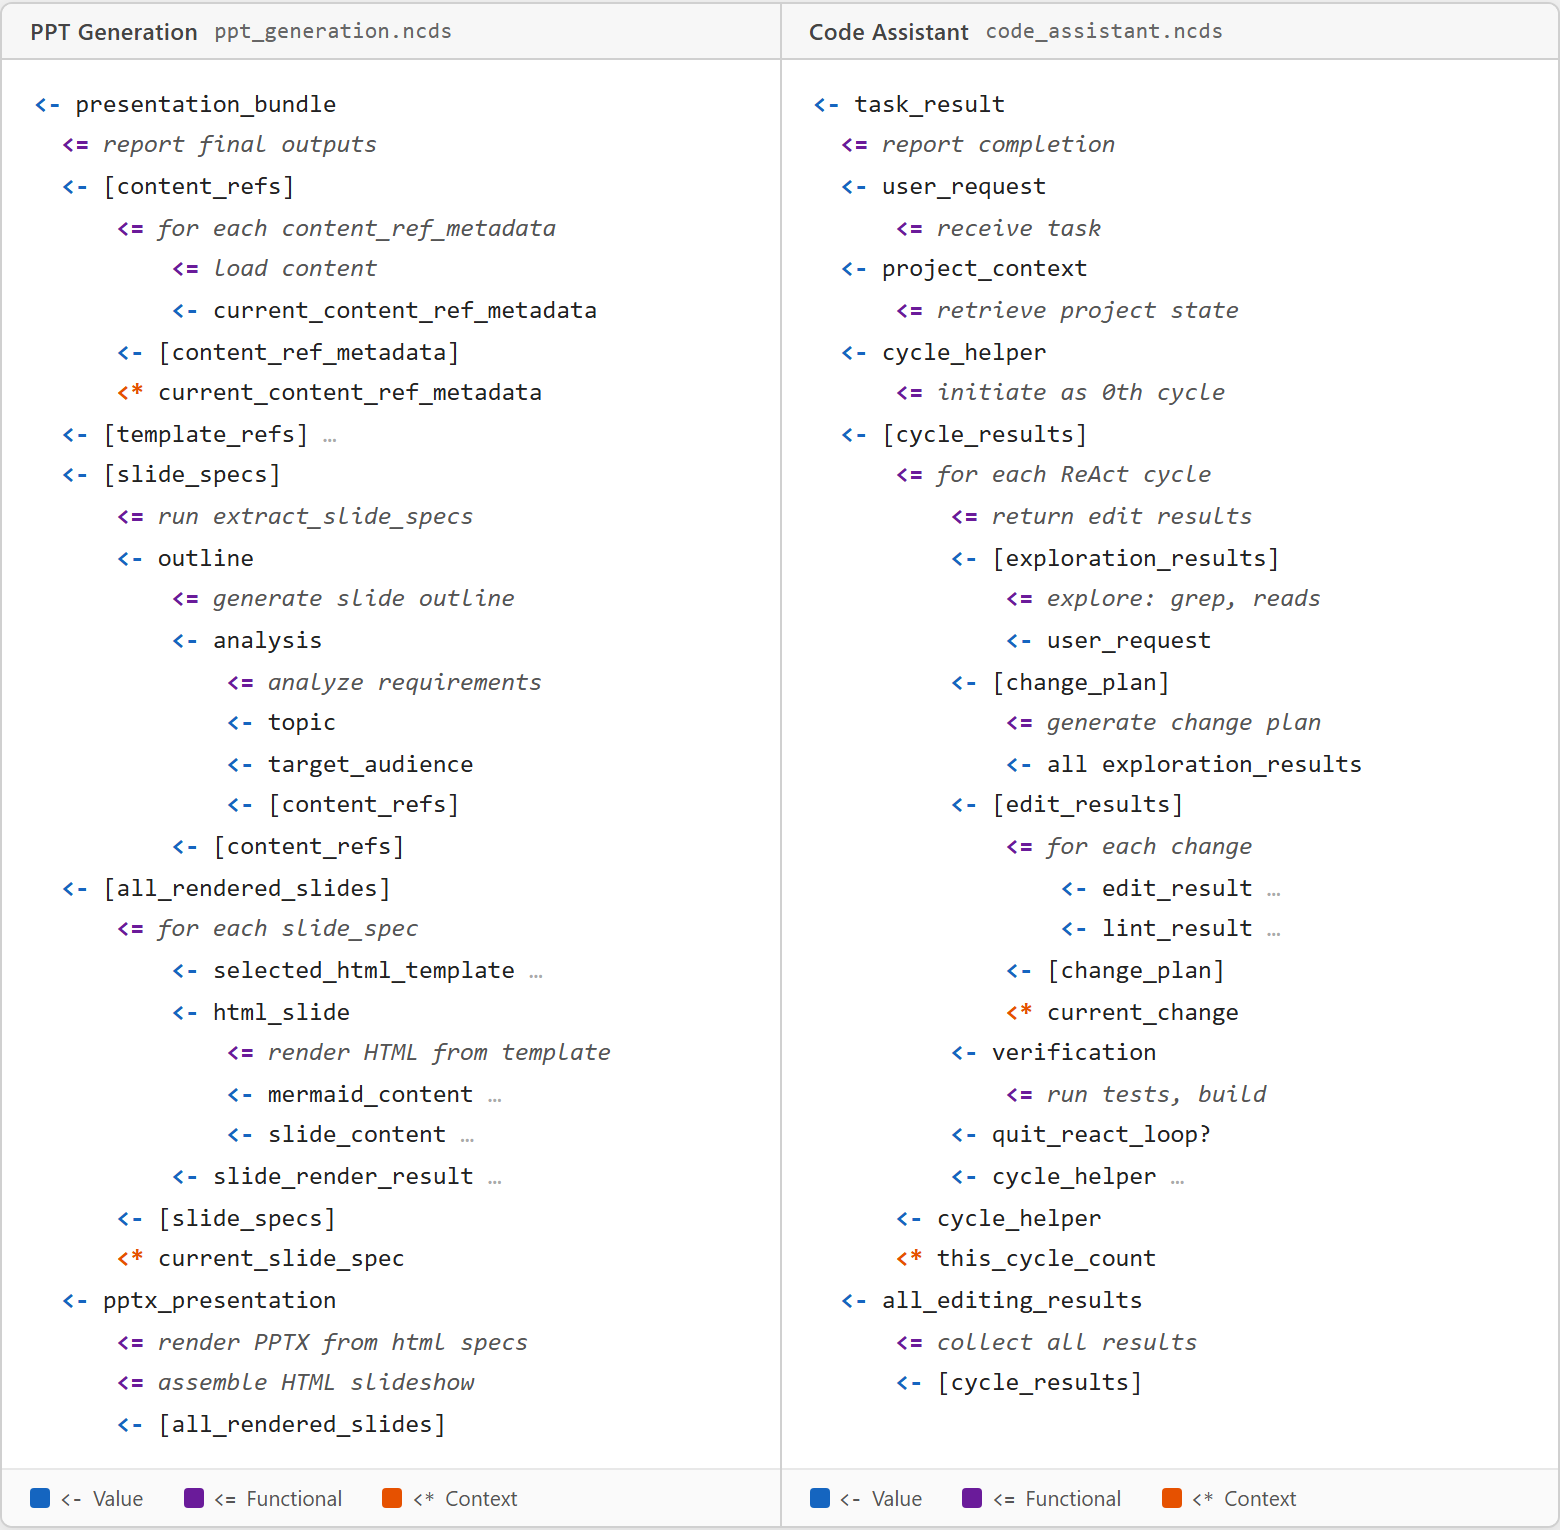
\includegraphics[width=\textwidth]{figures/ppt_and_code_ncs.png}
  \caption{PPT Generation (left) and Code Assistant (right) as Level~2 cases
    (\texttt{.ncds}, abbreviated).
    Left: nested dual-output loop (HTML + PPTX per slide).
    Right: ReAct outer loop \cite{yao2023} with inner explore, plan, edit, and verify stages.
    \textcolor{blue}{\texttt{<-}} Value; \textcolor{violet}{\texttt{<=}} Functional;
    \textcolor{orange}{\texttt{<*}} Context.}
  \label{fig:plans}
\end{figure}

\subsection{Case Study 1: PPT Agent --- Level 2 Reuse and Level 1 Accumulation}

\texttt{ppt\_generation.ncds} (Fig.~\ref{fig:plans}, left) is a Level~2 case encoding
a parallel dual-output pipeline: HTML and PPTX slides are generated from the same
componentized content JSON per slide. The most expensive semantic nodes are
\texttt{generate componentized content} and \texttt{generate diagram code};
the remainder run with negligible cost and a total latency around 5 minutes with
visible intermediate steps. The production plan uses Chinese concept names throughout
(Fig.~\ref{fig:ppt}); the compiler and orchestrator are agnostic to natural language.
Reusing a checkpoint requires the referenced files or APIs to remain accessible ---
the case encodes \textit{what} was used, not its content.

\begin{figure}[!htbp]
  \centering
  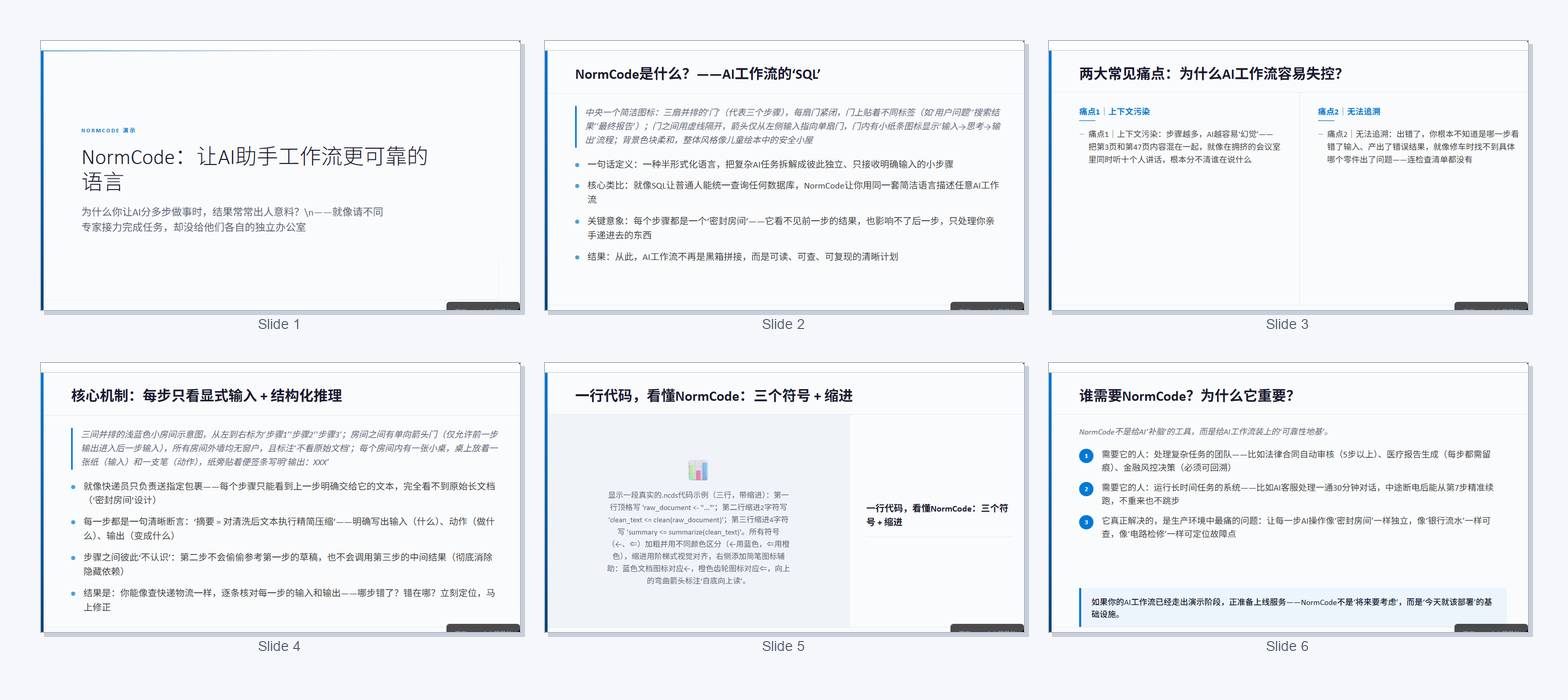
\includegraphics[width=\textwidth]{figures/fig4.png}
  \caption{Six slides produced by the PPT Generation plan (Chinese-language run).
    Each slide is a Level~1 checkpoint accumulated during execution.}
  \label{fig:ppt}
\end{figure}

\subsection{Case Study 2: Code Assistant --- A ReAct Plan as a Level~2 Case}

\texttt{code\_assistant.ncds} (Fig.~\ref{fig:plans}, right) is a Level~2 case encoding
a ReAct-loop software engineering workflow \cite{yao2023}. Each cycle, Explore
\textit{observes} (parallel file reads, zero LLM cost), Plan \textit{reasons} (one LLM
call over scoped exploration results), Implement \textit{acts} (surgical edits with an
inner lint-fix loop), and Verify checks results. Implement receives the change plan,
not the raw file contents from Explore --- scope isolation in action. Every run
generates a Level~1 case base: every stage is a checkpoint, and the Canvas App
makes each one inspectable and revisable (Sect.~\ref{sec:canvas}).



%================================================================
\section{Discussion}
\label{sec:discussion}

\textbf{Language as the substrate.} Failure localization (C1), pre-execution review
(C2), and selective re-execution (C3) are not design choices about the Canvas App. They
are structural consequences: (1)~C1 follows from Local Addressability --- every step
has an exact flow index; its inputs are exactly its declared scope. (2)~C2 follows from
Interpretability + Enforceability --- the \texttt{.ncn} is human-readable, and what the
reviewer reads is exactly what executes. (3)~C3 follows from Local Addressability +
Enforceability --- the scope rule determines which downstream nodes depend on any step;
the orchestrator enforces this boundary. Existing LLM orchestration tools can add
checkpoint UI features; they cannot produce these properties (C1--C3) structurally
without first providing a reasoning medium that satisfies these six properties.

\textbf{Sustainable improvement through two-level CBR.} (1)~\textit{Level~1
accumulation}: every run deposits concrete cases; past checkpoints are available for
retrieval, reuse, and revision without operator intervention. (2)~\textit{Level~2
refinement}: each domain that warrants a new plan extends the abstract case library;
plans are revised as task patterns evolve and retained. (3)~\textit{Recursive
improvement}: the compilation pipeline --- itself a Level~2 case --- improves through
the same revision cycle, producing better plans, better Level~1 cases, and better
Level~2 revisions in turn. This distinguishes NormCode from a logging tool: it
accumulates experience in a form that can be retrieved, reused, and improved
\cite{bergmann2002,muller2015b}.

\textbf{What CBR gains from a reasoning medium.} The scope rule, determined at compile
time and enforced at runtime, guarantees that every checkpoint is a self-contained case.
The Level~1 case definition extends POCBR's case representation
\cite{leake2008,bottrighi2016} to resumable execution environments: a trace records
what happened; a suspended runtime is a state from which execution can be continued
with exactly the same data-dependency behavior, providing a guarantee that trace
retrieval does not. Finally, this paper concretely deploys the two-level structure
introduced by Muller \& Bergmann \cite{muller2015b}: four abstract reasoning patterns
(Level~2) each generating concrete cases on every run (Level~1), with the compilation
pipeline itself a Level~2 case.

\subsection{Limitations}

\textbf{Operational limitations.} Case retrieval currently requires operator judgment to
select the appropriate fork target; learned similarity measures would lower this barrier.
The case base grows without bound --- competence-based pruning is a natural next step.
Semantic checkpoints (LLM outputs) are bounded-stochastic: same input produces the same
output distribution, not a fixed value. Checkpoints whose tensors contain perceptual
signs are structurally self-contained, but reuse requires the referenced external
resources to be accessible; the case encodes \textit{what was referenced}, not its
content.

\textbf{Methodological limitations.} The Derivation phase uses an LLM to extract
conceptual structure from natural language, introducing non-determinism in plan
generation; a more formal derivation procedure is a direction for future work.

\textbf{Evaluation scope.} Comprehensive quality evaluation would require a
combinatorial test matrix ($|L_2| \times |L_1|$ cells), where outcome quality also
depends on LLM model, input domain, and subjective judgment. The evaluation in
Sect.~\ref{sec:evaluation} therefore argues for Level~2 generalizability --- that the
structural properties hold across the four production plans and that C1--C3 (failure
localization, pre-execution review, selective re-execution) are realized --- rather than
for absolute output quality, which varies with domain, model
choice, and subjective criteria.




%================================================================
\section{Related Work}
\label{sec:related}

\subsection{Process-Oriented CBR Foundations}

The foundational CBR cycle was given its canonical formulation by Aamodt \& Plaza
\cite{aamodt1994}. Bergmann \cite{bergmann2002} provides foundational work on applying
CBR principles to workflow and experience management; Minor, Montani \& Recio-Garcia
\cite{minor2014} characterize POCBR as the field in which cases capture workflow
knowledge.

Within POCBR, Bergmann \& Gil \cite{bergmann2014} address efficient retrieval through
structural similarity; Muller \& Bergmann \cite{muller2015a} introduce a query language
where the query itself is a partial workflow. Bottrighi et al.\ \cite{bottrighi2016}
extend this to business process operational support. Leake \& Kendall-Morwick
\cite{leake2008} explicitly propose mining workflow provenance traces as CBR cases.
NormCode's contribution to this line of work is to provide a structural guarantee: by
enforcing scope isolation at the language level, every captured checkpoint is a
reliable, self-contained case rather than a trace that may embed implicit shared state.

\subsection{Multi-Level and Hierarchical CBR}

Muller \& Bergmann \cite{muller2015b} introduce generalized workflow cases that cover a
subspace of the case representation space --- the closest antecedent we are aware of to
NormCode's Level~2: both treat the abstract workflow pattern as a case object. The
generative difference is that NormCode's Level~2 cases are fully executable compiled
artifacts and the distillation process is itself expressible as a NormCode plan. Veloso
\cite{veloso1997} and Ihrig \& Kambhampati \cite{ihrig1997} establish that plan
derivations can be stored and retrieved as cases.

\subsection{CBR and Large Language Models}

Rubin, Herzig \& Berant \cite{rubin2022} learn to retrieve few-shot prompts; Wilkerson
\& Leake \cite{wilkerson2024} implement CBR components using LLMs; Lenz, Hoffmann \&
Bergmann \cite{lenz2025} evaluate LLMs as similarity assessors (LLsiM). These works use
CBR to improve individual LLM calls, or LLMs to implement CBR functions.

NormCode addresses a distinct problem: applying a CBR architecture to manage the
\textit{execution of multi-step LLM workflows}. Among prior work, Guo et al.\
\cite{guo2024} (DS-Agent) is the most directly related: CBR is used to iteratively
revise multi-step data-science plans. The structural difference is that DS-Agent's case
objects are narrative plans without enforcement guarantees, whereas NormCode's
checkpoints are structurally isolated by compiler and runtime --- which is the
precondition for reliable CBR retrieval and revision (Sect.~\ref{sec:background}).

\subsection{LLM Workflow Tools}

LangGraph provides checkpoint support and time-travel replay. PromptFlow and LangFlow
provide graph-based visual workflow authoring. AutoGen \cite{wu2023} supports
conversational multi-agent orchestration. These frameworks execute steps by passing
information through accumulated conversation histories or prompt templates that
implicitly reference prior outputs. Relative to NormCode's scope rule, none provides
explicit structural isolation guarantees at the language level: checkpoints may embed
implicit shared state from earlier steps. As a consequence, retrieving and replaying
such a checkpoint in a new execution context may produce incorrect behavior, failures
are non-localizable, and case reuse is not guaranteed to reproduce the original
data-dependency behavior --- the three conditions identified in
Sect.~\ref{sec:background} as preconditions for reliable CBR operations.

\subsection{LLM Agents and the ReAct Pattern}

Yao et al.\ \cite{yao2023} propose ReAct --- interleaving reasoning traces with
grounded action execution in a tight loop. The observe-reason-act pattern has since
become a standard building block for tool-using LLM systems. Reflexion
\cite{shinn2023} extends it with verbal reinforcement: agents verbalize failure
feedback into episodic memory and retry, improving without weight updates. MetaGPT
\cite{hong2024} encodes software-engineering standard operating procedures as prompt
sequences for multi-role agent collaboration; SWE-agent \cite{yang2024} introduces an
agent-computer interface for autonomous software engineering. AutoGen \cite{wu2023}
generalizes the pattern to conversational multi-agent coordination.

NormCode plans that use Canvas Integration facilities implement the ReAct pattern as
explicitly compiled plans. The Canvas Assistant's per-iteration loop --- read user
input $\rightarrow$ classify command $\rightarrow$ execute via \texttt{me.hands} or
\texttt{me.mind} $\rightarrow$ generate response --- is a ReAct cycle expressed as a
structured plan with declared scopes. The Code Assistant's pipeline similarly reasons
over retrieved context and acts via tool calls across seven stages.

Deployed agentic coding tools --- Cursor \cite{cursor2024}, Claude Code
\cite{claudecode2026}, and OpenClaw \cite{openclaw2026} --- demonstrate this pattern
at production scale: each implements a persistent observe-reason-act loop over
codebases, terminals, and file systems. The core workflow of such tools --- triage the
task, explore context, generate and apply changes, verify --- is structurally similar
to the Code Assistant NormCode plan. Expressed as a NormCode Level~2 case, this
workflow gains auditable structure, pre-execution review (C2), and a Level~1 case base
at every agent step. The NormCode framing is therefore not specific to the four plans
presented here; it applies to the class of deployed agentic tools at large.

The structural difference is that in standard ReAct and its derivatives, the
reasoning-action chain is an implicit continuation; the reasoning trace and runtime
state are not formally separated. In NormCode, each step in the agent loop is a node
with a declared scope, a flow index, and an automatic checkpoint. The agent's execution
trace is a Level~1 case base: every iteration step is inspectable, revisable, and
reusable under the CBR operations C1 and C3. The absence of this property in existing
frameworks is independently confirmed by recent work: AgentStepper \cite{agentstepper2026}
introduces post-hoc interactive debugging (breakpoints, step-through, online prompt
editing) for software development agents precisely because the underlying frameworks
provide no structural transparency. NormCode makes these properties structural rather
than retrofitted.

\subsection{Process Mining}

Process mining \cite{vandermaaist2011} discovers process models from event logs.
NormCode's Level~2 distillation is related in spirit to guided process model discovery.
The key difference is authorial intent: process mining performs automated discovery from
logs, while NormCode's compilation is human-directed and LLM-assisted, producing
executable artifacts rather than descriptive models.


%----------------------------------------------------------------
\newpage
\begin{credits}
\subsubsection{\ackname} Acknowledgements will be added in the camera-ready version after blind review.

\subsubsection{Declaration on Generative AI}
During the preparation of this work, the author(s) used AI-assisted writing tools for
drafting and editing. After using these tools, the author(s) reviewed and edited the
content as needed and take(s) full responsibility for the publication's content.
\end{credits}

\bibliographystyle{splncs04}
\bibliography{bibliography}

\end{document}
